
\section{More figures}

This section includes some examples of different types of figures to include. A simple single figure is shown in figure \ref{fig:trajectory_angle}, while figure \ref{fig:cyclic} shows how three subfigures can be included together. Remember to change both the caption and the title in the square brackets before the caption, which will show up in the list of figures. \\

\noindent page fill page fill page fill page fill page fill page fill page fill page fill page fill page fill page fill page fill page fill page fill page fill page fill page fill page fill page fill page fill page fill page fill page fill page fill page fill page fill page fill page fill page fill page fill page fill page fill page fill page fill page fill page fill page fill page fill page fill page fill page fill page fill page fill page fill page fill page fill.

\begin{figure}[H]
  \centering
  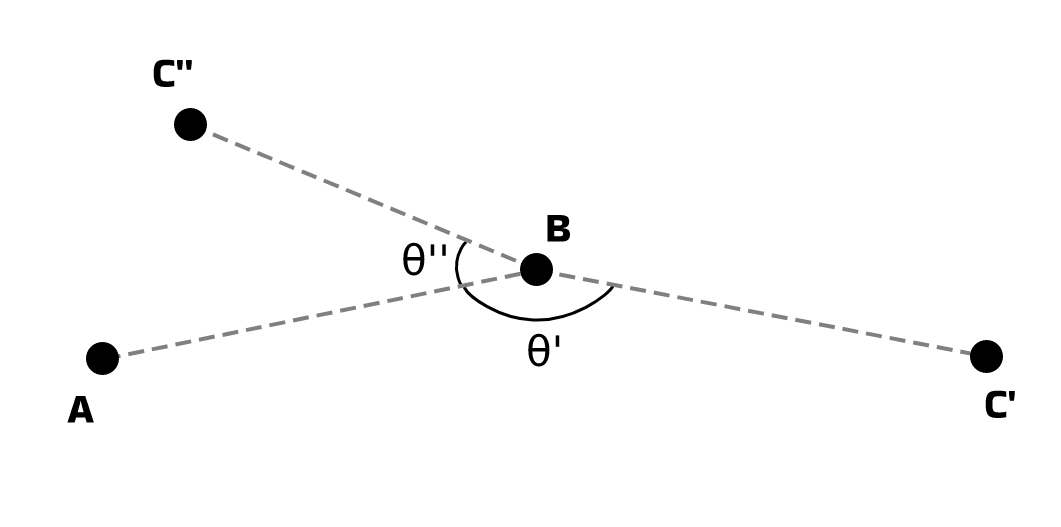
\includegraphics[width=1\textwidth]{Figures/trajectory angle.png}
  \caption[Trajectory angle]{The trajectory angle found for the trajectory ABC between the three points A, B and C. The two different C-points show the angle gotten for relatively unchanged directional trajectory with C', and opposite directional trajectory with C''.}
  \label{fig:trajectory_angle}
\end{figure}



\begin{figure}[H]
  \centering
  \subfloat[Time as a linear variable.]{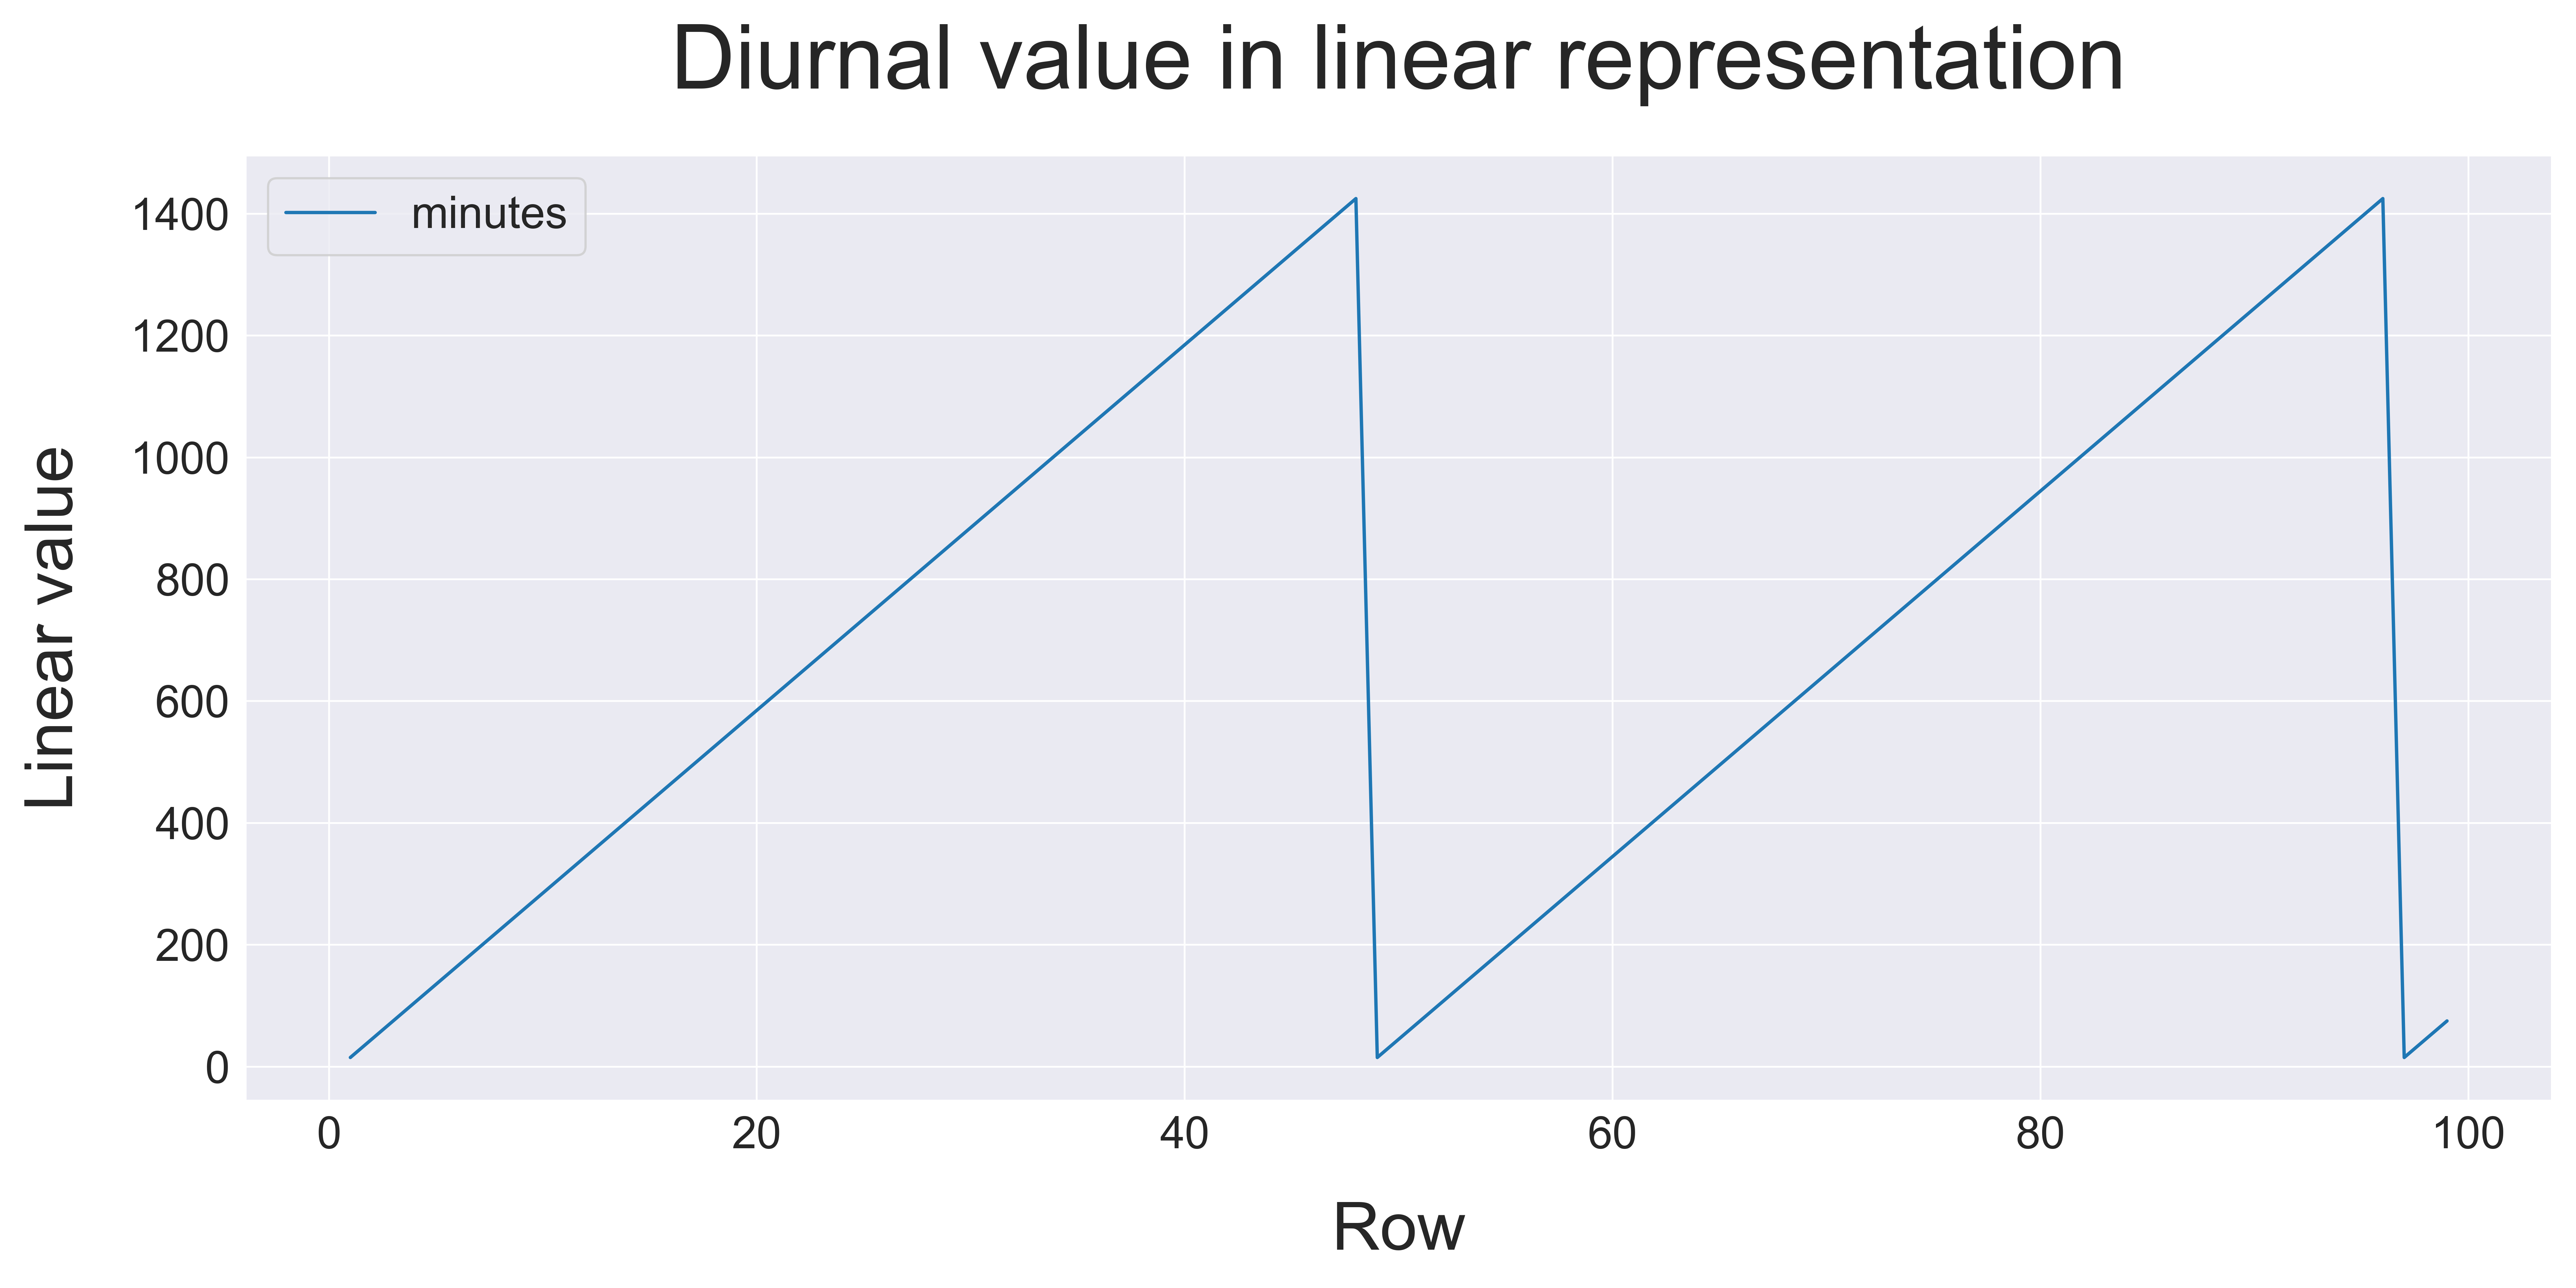
\includegraphics[width=0.75\textwidth]{Figures/diurnal_values_linear.png}\label{fig:diurnal_lin}}
  \hfill
  \subfloat[Time represented as pairs of sine and cosine.]{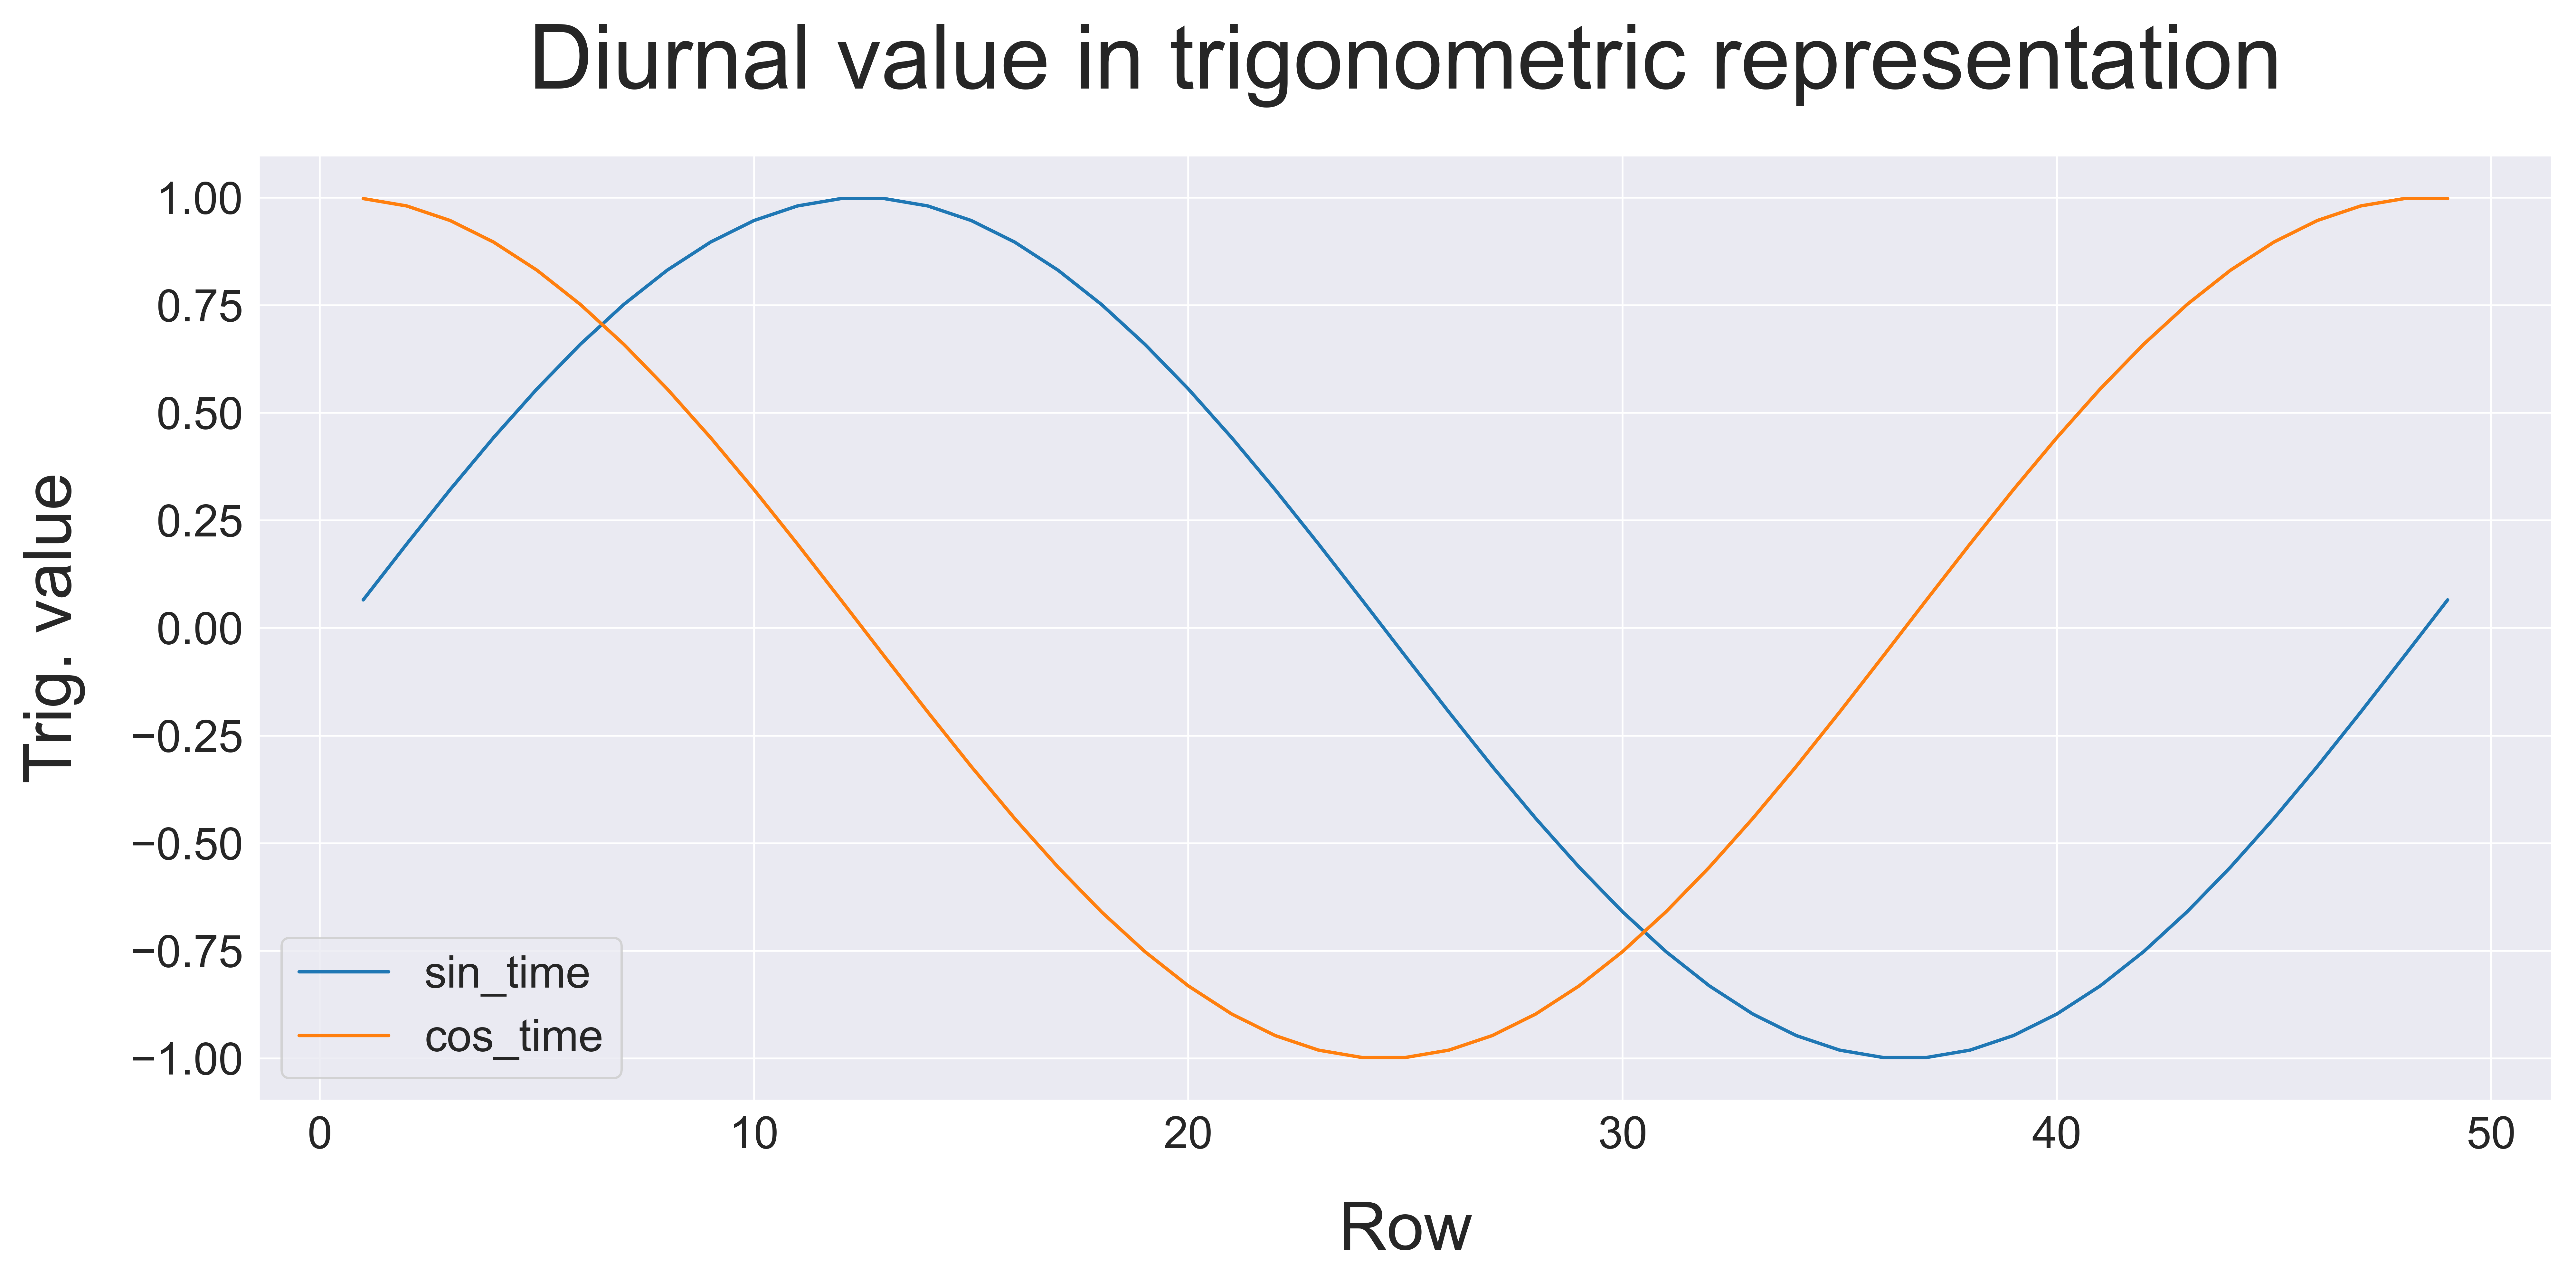
\includegraphics[width=0.75\textwidth]{Figures/diurnal_values_sine.png}\label{fig:diurnal_trig}}
  \hfill
  \subfloat[Time as a cyclic feature.]{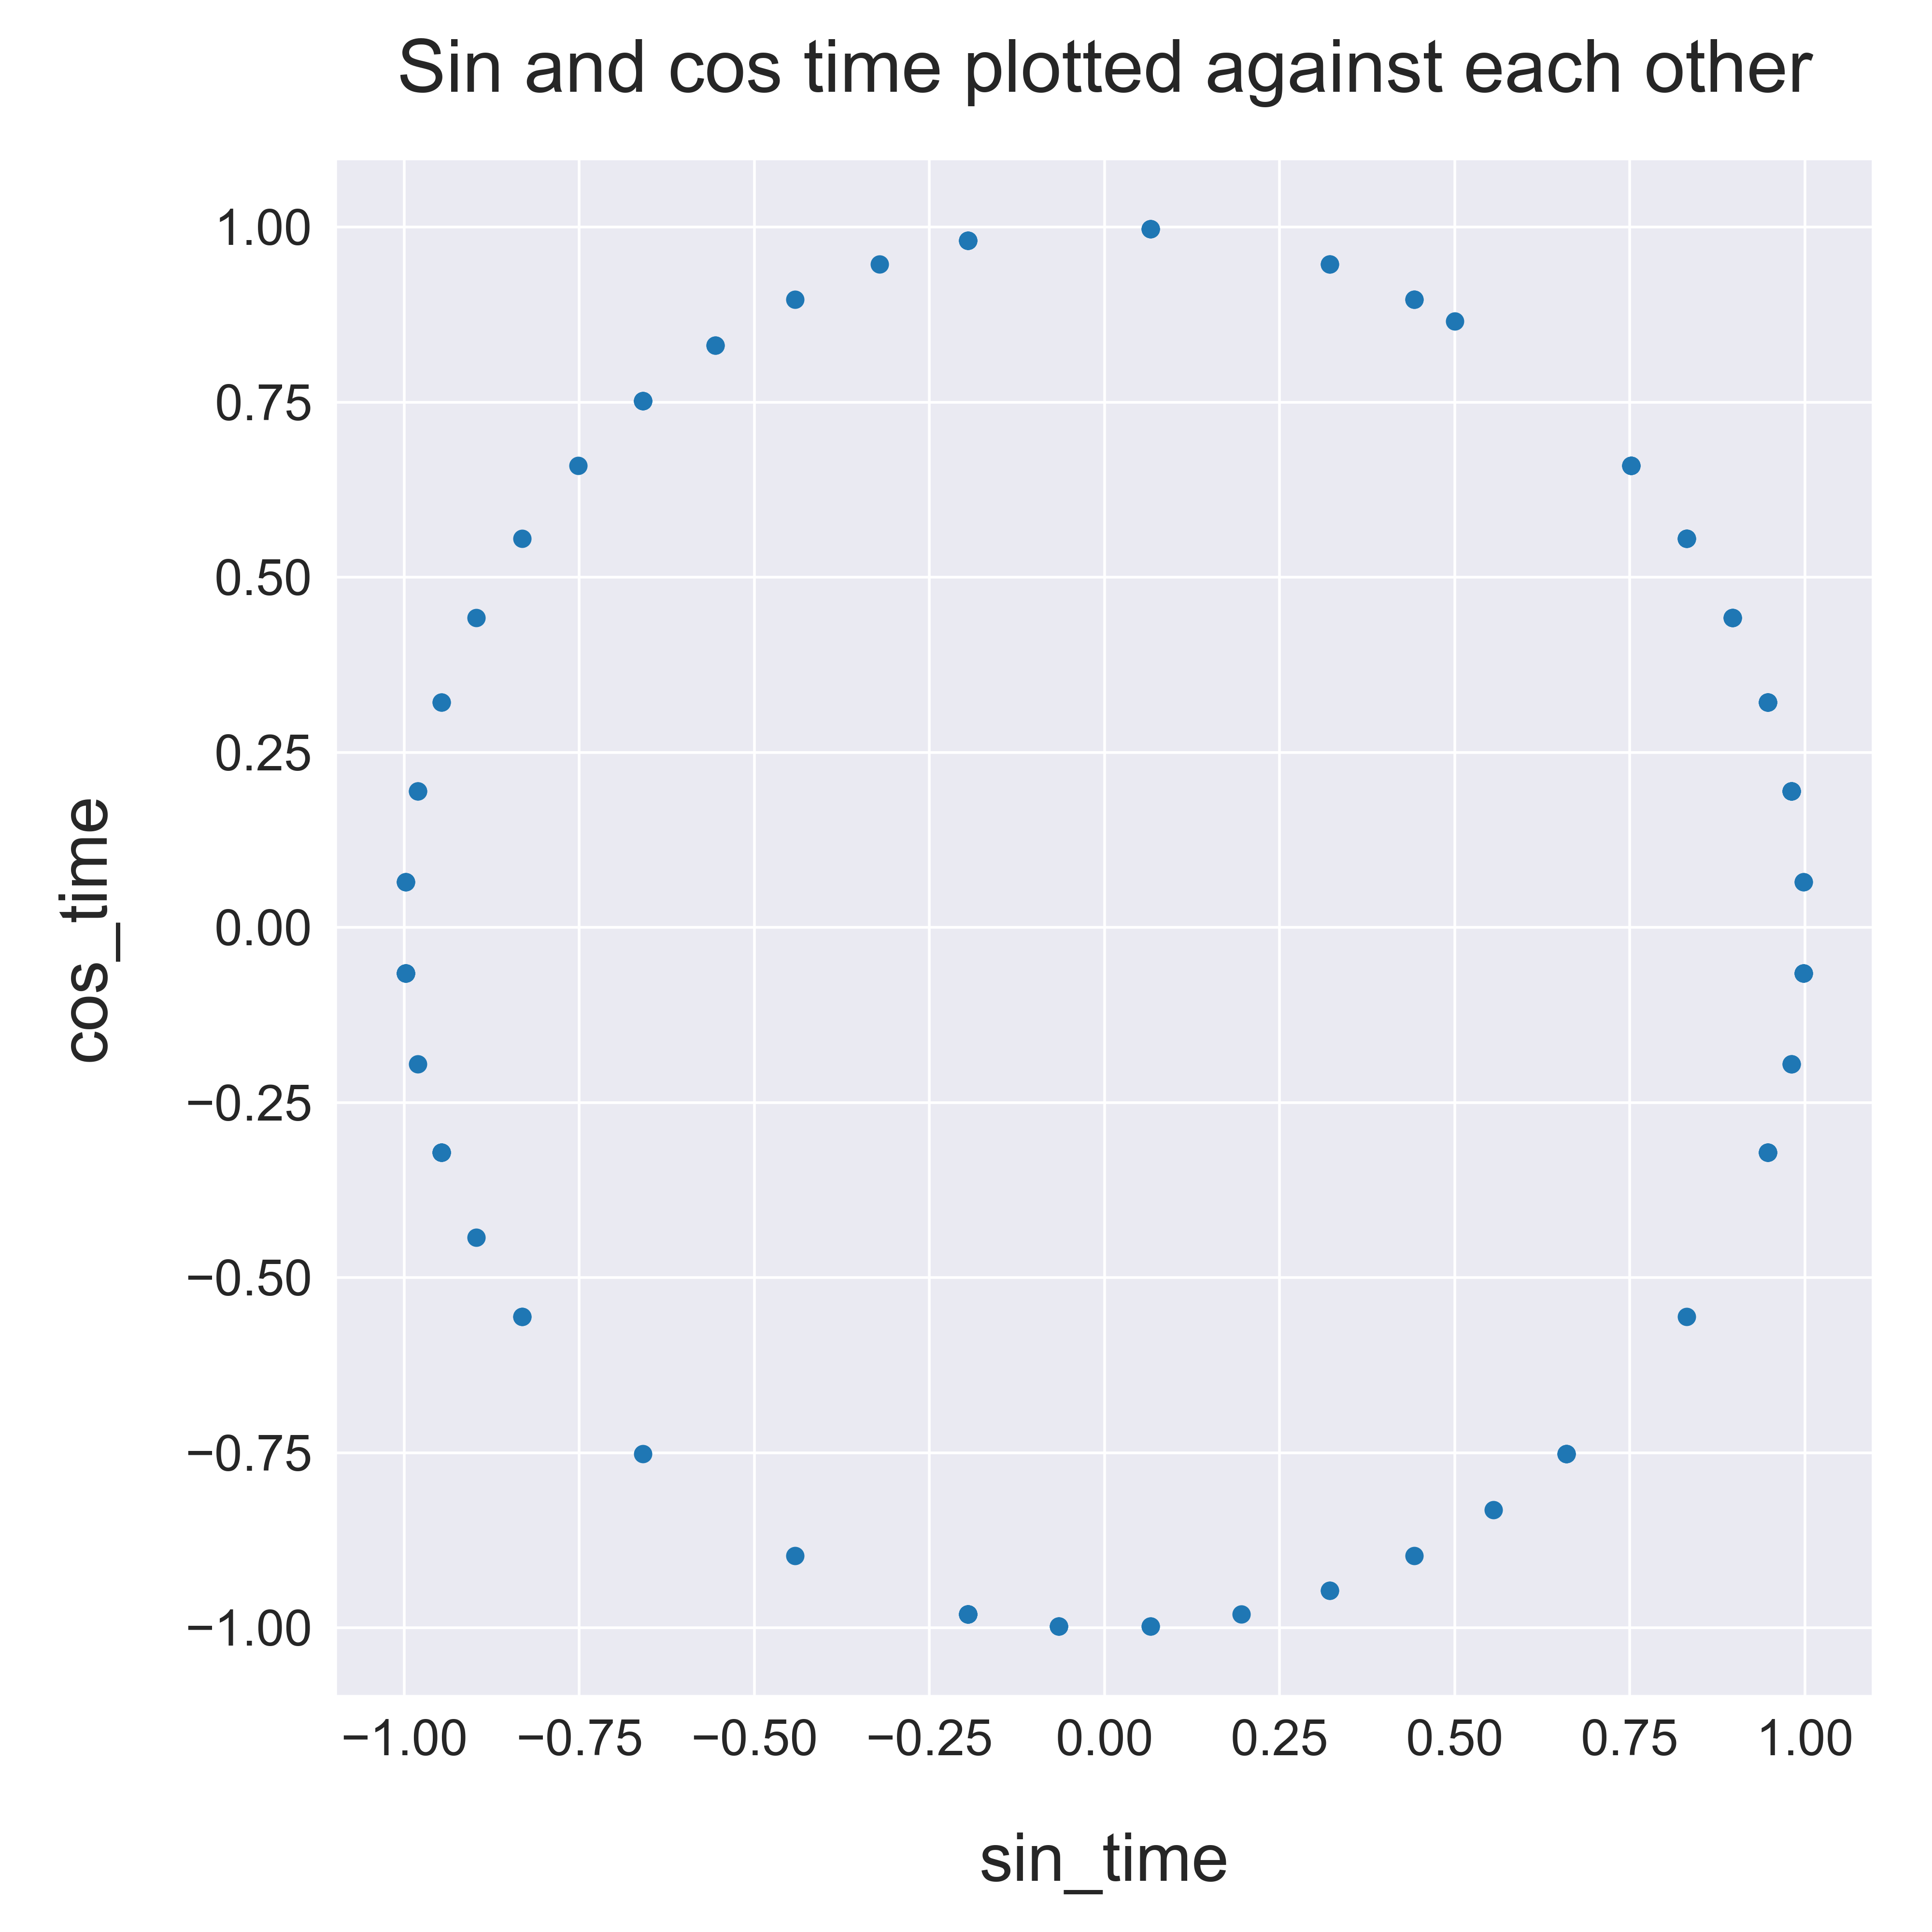
\includegraphics[width=0.6\textwidth]{Figures/diurnal_values_circle.png}\label{fig:diurnal_cyclic}}
  
  \caption[Time as a cyclic feature]{Figure (a) shows the time variable in the data for the first 100 rows using linear time as minutes past midnight, figure (b) shows the trigonometric time representation for one cycle where each time point has a unique sine and cosine-pair value, and figure (c) shows time as a cyclic feature with the trigonometric pairs.}
\label{fig:cyclic}
\end{figure}